\documentclass[11pt,a4paper]{article}

% ------------------------------------------------------------
% PACKAGES
% ------------------------------------------------------------
\usepackage[a4paper,left=20mm,right=20mm,top=20mm,bottom=20mm]{geometry}
\usepackage{amsmath}
\usepackage{amssymb}
\usepackage{siunitx}
\usepackage{graphicx}
\usepackage{float}
\usepackage{array}
\usepackage{tabularx}
\usepackage{longtable}
\usepackage{booktabs}
\usepackage{caption}
\usepackage{xcolor}
\usepackage{listings}
\usepackage[hidelinks]{hyperref}

% ------------------------------------------------------------
% FORMATTING
% ------------------------------------------------------------
\setlength{\parindent}{0.5cm}
\setlength{\parskip}{0.4em}

\newcolumntype{Y}{>{\raggedright\arraybackslash}X}
\newcolumntype{L}[1]{>{\raggedright\arraybackslash}p{#1}}

\lstset{
	basicstyle=\ttfamily\scriptsize,
	breaklines=true,
	columns=fullflexible,
	frame=single,
	keepspaces=true,
	tabsize=4,
	showstringspaces=false,
	numbers=left,
	numberstyle=\tiny
}

% ------------------------------------------------------------
% DOCUMENT INFORMATION
% ------------------------------------------------------------
\title{Design (E) 314 Test 4 Study Notes}
\author{Student Name}
\date{\today}

\begin{document}
	
	% ------------------------------------------------------------
	% TITLE PAGE
	% ------------------------------------------------------------
	\begin{titlepage}
		\centering
		\vspace*{0.5cm}
		
		\rule{\linewidth}{0.2mm}\\[0.4cm]
		{\huge \bfseries Skripsie Progress Report}\\[0.4cm]
		\rule{\linewidth}{0.2mm}\\[1.5cm]
		
		\begin{minipage}{6.5cm}
			\begin{flushleft}
				\large
				\emph{Author:}\\
				Karl Johan Hofmeyr
			\end{flushleft}
		\end{minipage}
		~
		\begin{minipage}{6.5cm}
			\begin{flushright}
				\large
				\emph{Student Number:}\\
				27150526
			\end{flushright}
		\end{minipage}
		
		\vspace{2cm}
		{\large \today}
		
		\vfill
	\end{titlepage}
	
	\pagenumbering{arabic}
	\newpage
	
	% ============================================================
	\section{Work Completed}
	% ============================================================
	
	The building and testing of the equaliser has been completed. Equiliser is functioning as intended and can be finalised.
	
	\begin{figure}[h]
		\centering
		\href{run:demo.mp4}{
			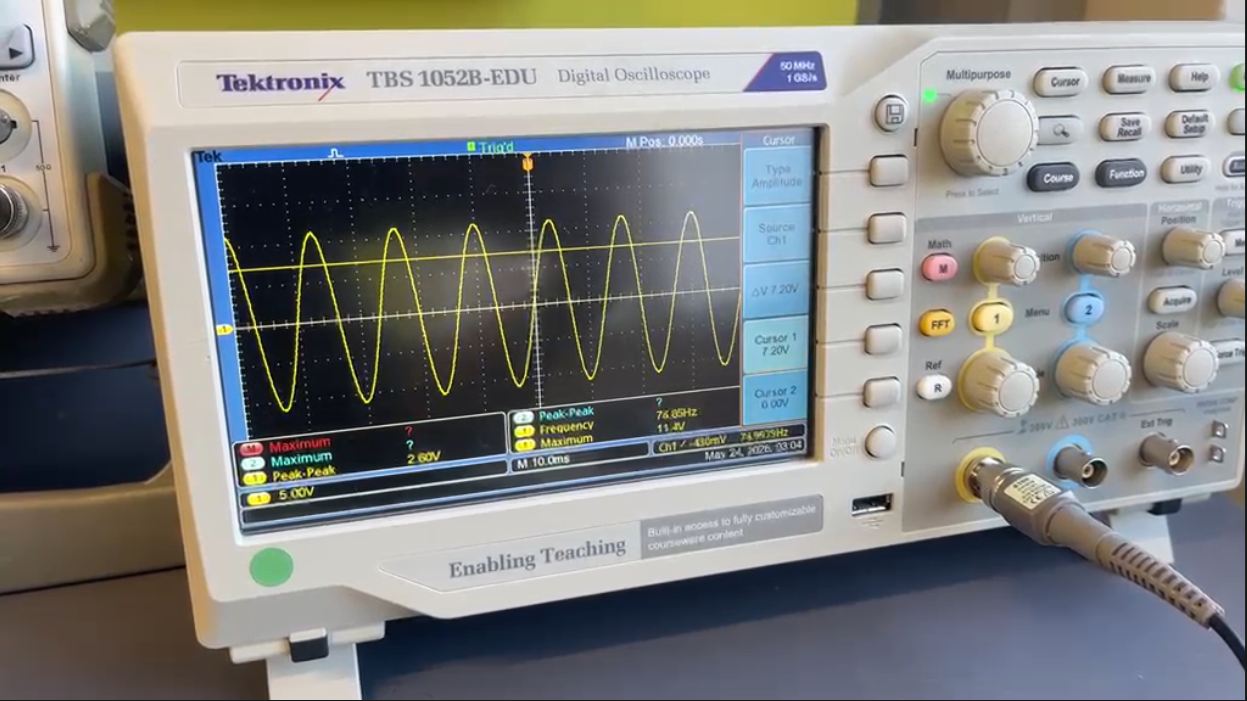
\includegraphics[width=0.7\textwidth]{video-preview.png}
		}
		\caption{Adjustment of Bass at 75Hz}
	\end{figure}
	
	The equaliser circuit has been changed to fit the design better. New design also uses less components, and has lower THD.
	
	\begin{figure}[h]
		\centering
		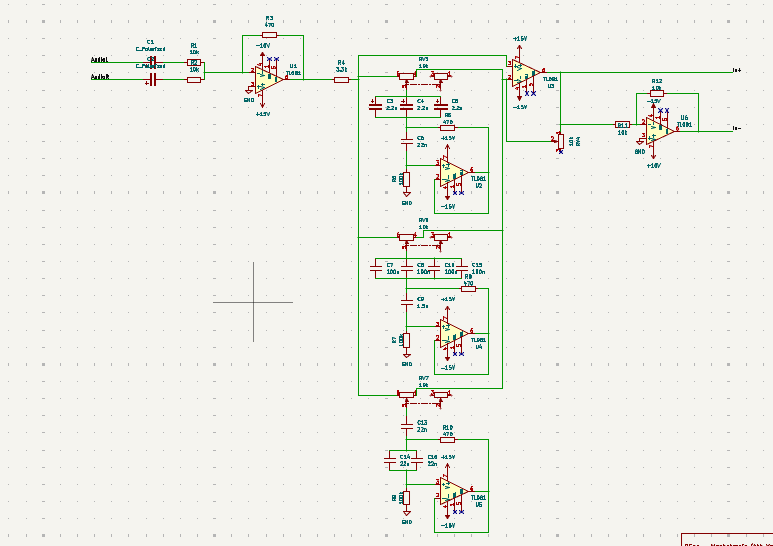
\includegraphics[width=0.7\textwidth]{equiliserAdjusted.png}
		\caption{Redesigned and tested equaliser circuit}
	\end{figure}
	
	\newpage
	The regulator circuits for the STM32, fans, equaliser and display have been designed
	
	\begin{figure}[h]
		\centering
		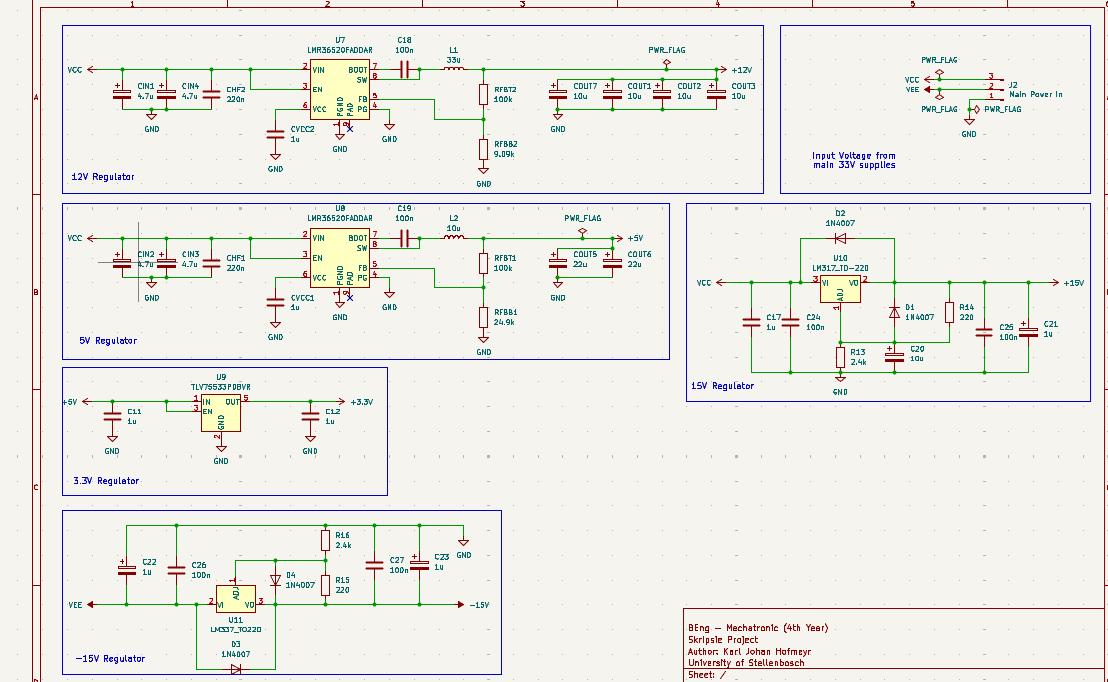
\includegraphics[width=0.7\textwidth]{regulators.png}
		\caption{Voltage Regulator Circuits}
	\end{figure}
	
	The pinout for the stm32 has been chosen
	
	\begin{figure}[h]
		\centering
		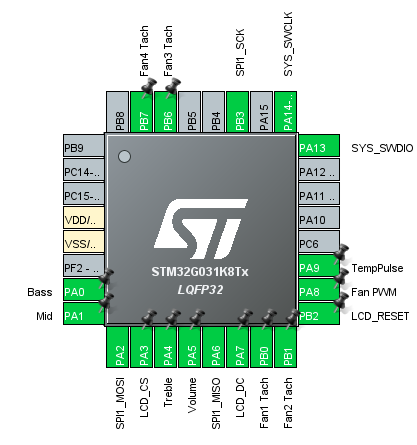
\includegraphics[width=0.7\textwidth, height=0.6\textwidth]{pinout.png}
		\caption{STM32 pinout setup}
	\end{figure}
	
	\newpage
	
	\section{Work to Complete}
	
	\begin{itemize}
		\item Complete schematics
		\item Finalise BOM materials and order components
		\item Start PCB designs
		\item Heat calculations for heat sink
		\item Possibly design linear power supply, better than switch mode
	\end{itemize}
	
\end{document}
